
%(BEGIN_QUESTION)
% Copyright 2012, Tony R. Kuphaldt, released under the Creative Commons Attribution License (v 1.0)
% This means you may do almost anything with this work of mine, so long as you give me proper credit

A technician is asked to build a recording system to continuously monitor the position of a control valve's stem.  Her solution is to connect a resistor in series with the I/P converter's 4-20 mA current signal, then connect a voltage-registering trend recorder to graph the signal over time:

$$\includegraphics[width=15.5cm]{i03405x01.eps}$$

Finish connecting the wires from the recorder to the I/P circuit so that it will be able to record the control signal.

Next, write a mathematical formula calculating the position of the valve as a function of the voltage received by the recorder.  This formula will be entered into the digital recorder so that it can display an actual percentage value on the trend (between 0\% and 100\% valve position) and not just a voltage value.  In other words, this formula should have one unknown variable ($V$) as its only ``input,'' and ``output'' a percentage value indicating the position of the control valve (between 0\% and 100\% open):

\vskip 20pt

Valve position (\%) = 

\underbar{file i03405}
%(END_QUESTION)





%(BEGIN_ANSWER)

I recommend half-credit for the completed sketch and half-credit for the formula:

$$\includegraphics[width=15.5cm]{i03405x02.eps}$$

\vskip 10pt

Valve position (\%) = $0.52083 V - 0.25$ (percentage expressed as a number 0-1)

Valve position (\%) = $52.083 V - 25$ (percentage expressed as a number 0-100) 

%(END_ANSWER)





%(BEGIN_NOTES)

{\bf This question is intended for exams only and not worksheets!}.

%(END_NOTES)


